\documentclass[10pt]{article}
    \usepackage{graphicx}
    \usepackage{amsmath}
    \usepackage{mathptmx}
    \usepackage{dblfloatfix}
    \usepackage{newfloat}
    \usepackage{listings}
    \DeclareFloatingEnvironment[name={Figure}]{suppfigure}
    \setcounter{suppfigure}{1}
    \usepackage[top=1.75cm, bottom=1.75cm, left=1.75cm, right=1.75cm, a4paper]{geometry}
    \setlength{\columnsep}{1cm}
    \graphicspath{ {./businessImages/} }
    \lefthyphenmin4
    \righthyphenmin4
    \emergencystretch=1cm
    
    \begin{document}
    
    \begin{titlepage}
        \begin{center}
        \vspace*{1cm}
    
        \Large
        \textbf{An Actor-Critic implementation for solving platform games on SpiNNaker}
    
        \vspace{0.5cm}
            Stefan Grigore
    
        \vspace{0.5cm} 
        
            Supervisor: Prof. Steve Furber

        \vspace{0.5cm} 

            April 2019
    
        \vspace{1.5cm}

        \vfill

        Third Year Project Report \\
        MEng Computer Science \\
        School of Computer Science - University of Manchester
     
        \end{center}
    \end{titlepage}

    \twocolumn
    
    \textbf{\textit{Abstract} --- Translating high level environmental inputs to meaningful actions and strategies is an important problem for fields such as mobile robotics or robotic prostethics. Some of the greatest obstacles faced are the number of iterations that conventional learning models require to produce effective strategies, and the unpredictable results that actions in the real world have. Furthermore, encoding these strategies and retrieving resulting actions require complex data structures that pose limitations regarding scalability, power consumption, memory use and computational time for elaborate tasks performed by embedded systems. This report describes an implementation on the SpiNNaker neuromorphic computing platform of an Actor-Critic inspired model, applied to solve a platform game that outlines the problems a real world task might present. The project aims to use the SpiNNaker platform to tackle the obstacles of such applications, and to produce a biologically plausible model that might give an insight into how learning and memory work in the human brain.}

    \textbf{Key Words: actor-critic methods, reinforcement learning, spiking neural networks}


    \tableofcontents
    \section{Introduction}
    
    The main limitations of neural network implementations is scalability, power consumption, memory use and computation time. The chip area required by synapses increases quadratically with the number of neurons (Benjamin et al., 2014). Furthermore, the computational complexity, memory and power consumption of the model grows with the precision of the simulation (the firing rate of neurons) as each signal needs to be propagated across the network to alter the synaptic weights (Brette et al., 2007). All these factors pose problems for models that aim to solve complex, faster than real time tasks as part of embedded systems. The motivation behind pursuing a biologically plausible model and using a platform such as SpiNNaker is also inspired by the great discrepancy of several orders of magnitude (Sarpeshkar, 1998) in computational efficiency between neurobiology and electronics, which has been first pointed out by Mead (Mead, 1990).

    \begin{suppfigure*}[b]
    \center
    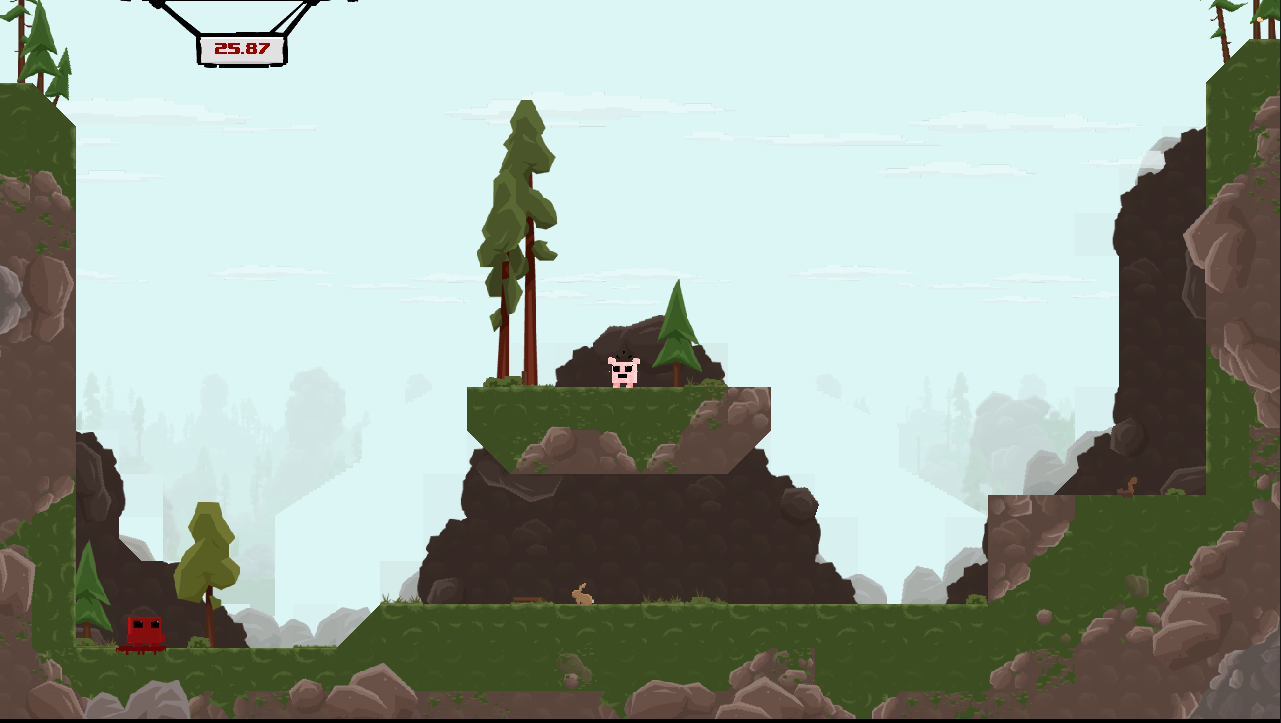
\includegraphics[width=165mm]{./level1.png}
    \caption{Frist level of Super Meat Boy, with the red, square shaped main character on the bottom left and the pink goal on the middle platform}
    \label{fig:firstLevel}
    \end{suppfigure*}

    \subsection{Project goals}

    The scope of this project is to produce a high performance, high scalability, customisable and biologically plausible spiking neural network reinforcement learning model that solves pathfinding and platform games in a limited number of learning episodes, and that could be adapted for other tasks such as controlling hardware with the purpose of reaching similar learning and progress-based goals.

    One important aim of the project is to gain practical experience and an understanding of neuromorphic computing and spiking neural networks that would give an inshight into how the human brain works and how this knowledge can help us build more efficient software systems.

    The report will detail the different approaches for managing, representing and extracting information from spiking neural networks, the ability of the model to learn and adapt, the performance of the model, limitations of the platform and possible future developments.

    \section{Background}

    This section introduces the characteristics of the SpiNNaker board that was used to develop this project, the reinforcement learning model that was implemented and the game chosen to showcase this model.

    \begin{suppfigure*}[b]
    \center
    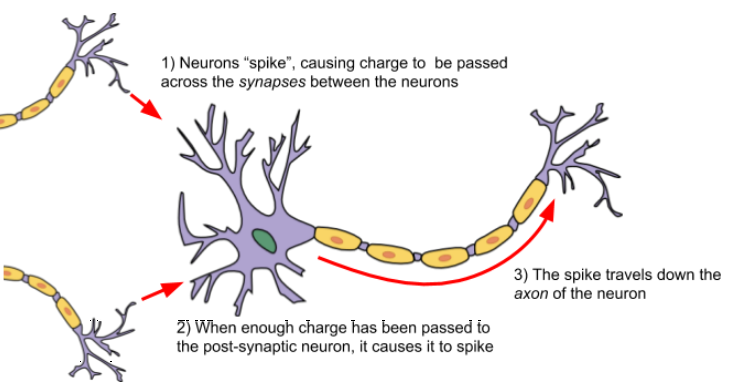
\includegraphics[width=150mm]{./neurons.png}
    \caption{Neuron and myelinated axon, with signal flow from inputs at dendrites to outputs at axon terminals (SpiNNaker Manchester, 2016)}
    \label{fig:neurons}
    \end{suppfigure*}

    \subsection{The SpiNNaker system}

    SpiNNaker (Furber et al., 2014) is a massivelly parallel, event-based neuromorphic computing platform composed of low-power ARM processors which enables the real time simulation of spiking neural networks. The advantage of a spiking neuron over models such as the fully digital, first generation perceptron model or the second generation sigmoidal neural net is that it describes the output of a biological neuron more accurately by incorporating the concept of time in order to encode information (Maass, 1996). The application presented in this report has been implemented by using a 4 node SpiNN-3 board. Each node is composed of 18 processing cores, one of them elected at start-up as a Monitor Core, leaving 16 cores to support the application and one left for fault tolerance and manufacturing yield enhancing purposes (Furber et al., 2013). Each core can model around 1000 neurons, such as the leaky integrate and fire model, which simulates the loss of potential that occurs at the membrane level of the biological neuron.

    \begin{figure}[ht!]
    \centering
    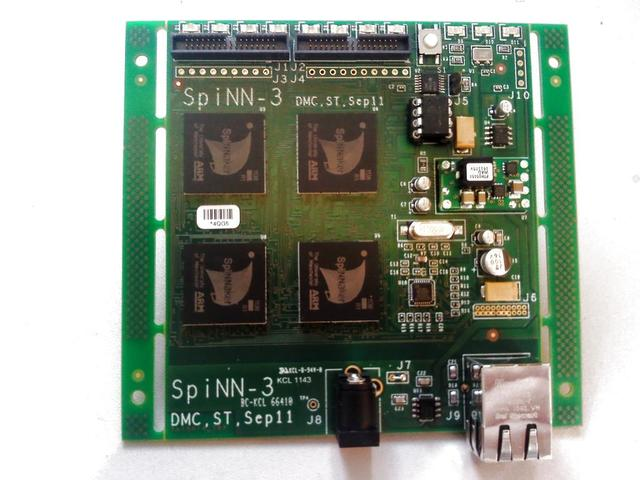
\includegraphics[width=80mm]{./SpiNN-3.jpg}
    \caption{A 4-node SpiNN-3 board \label{overflow}}
    \label{fig:spinnBoard}
    \end{figure}

    \setcounter{figure}{3}

    The supporting software provided is the sPyNNaker Python library which enables the specification of neural models using the PyNN description language, and the run-time user interaction with the simulation.

    The Python programs produced can be either run on a local board such as the one shown in Figure \ref{fig:spinnBoard}, or they can be submitted as jobs to a remote SpiNNaker server that would execute them and give back results. The latency of the communication with such a server, however, would not be suitable for the real time interaction that is done with the system for this project, so it has been implemented by using the local SpiNN-3 board which is connected to the computer hosting the Python application via an Ethernet interface.

    \subsection{The game}

    The game chosen to showcase the learning model is called Super Meat Boy, a commercially available video game developed by independent studio Team Meat. The game belongs to the genre of platform games, where a player controlled character has to jump and climb between suspended platforms while avoiding obstacles in order to reach a goal.   

    The game was chosen because it showcases some of the properties of the gridworld task (Sutton et al., 1998), used as a common test case for reinforcement learning. The character can move in the 4 directions of the 2D plane, with the addition of properties such as gravity, intertia or friction. These additional elements mean that the movements are not precise, and the actions of the agent do not always go as planned. There are also no pre-built tools for simulating the game to speed up the training of the model over many episodes for tabular learning methods such as Q-Learning or SARSA. All these aspects highlight problems that real-world application have to tackle.

    \subsection{Reinforcement Learning}

    Supervised learning models learn from labeled examples and with the use of a "knowledgeable teacher". They aim to gradually decrease the deviation (error) between the target output and actual output of the model. Compared to this method, reinforcement learning models use a "critic" which does not need to have knowledge of the target output. The critic only evaluates the behaviour of the system based on environmental inputs, and the model aims to maximise the amount of reward and decrease the amount of penalty. This mimics the behaviour described in the theory which states that neurons are individually "hedonists" that work to maximise a local analog of pleasure, while minimizing a local analog of pain (Klopf, 1982). Furthermore, experiments found that animals learn through an "associative process", where by trial and error over repeated iterations they can find the optimal solution to puzzles (Thorndike, 1898). In these experiments it was found that actions closely followed by satisfaction become more likely to occur, while those which are accompanied by discomfort become less likely (the law of effect).

    Reinforcement learning exploits actions that worked best for each situation while searching new actions through trial and evaluation.
    
    \section{Development}

    This chapter covers the library used to implement the model and the biological analogues behind its components and behaviour. Furthermore, this section provides an in-depth description of the architecture of the model and the reasoning behind it. The architecture is inspired by a spiking implementation of an actor critic learning agent already described by Potjans et. al, 2009. Parallels are made to this source, while also presenting novel ideas for encoding the policy of the agent and adapting the techniques described in the paper to the SpiNNaker platform.

    \subsection{The sPyNNaker Python library}

    The project has been implemented by using the sPyNNaker Python library which enables the modelling of spiking neurons and neural networks, the simulation of those models and the run-time interaction with them (Rhodes et al., 2018).

    \subsubsection{Spiking neural networks}

    Biological neurons have been observed to produce sharp increases in electrical potential across their membrane, lasting roughly 1 millisecond, commonly known as spikes. As charges are transferred across synapses from pre-synaptic neurons to a post-synaptic one, the potential of the post-synaptic neuron builds up until it releases the charge itself in the form of a spike that is sent forward in the network, where the process repeats.

    The library uses the PyNN neural network description language to build the models of these neurons and the interactions between them. Neural populations are created, representing groups of neurons with similar properties. A number of standard neuron models are provided by PyNN, with one of the most basic of them being the Leaky Integrate and Fire (LIF) model. The LIF neuron is modeled as a resistor and capacitor connected in parallel. Charge is built in the capacitor as spikes are received, but leaks out through the resistor over time. If the voltage exceeds a threshold, the charge is released in the form of a spike which is transmitted to the connected post-synaptic neurons. Once a refractory period where the neuron is not allowed to spike again passes, the neuron resumes operation as before (Rhodes et al., 2018). 
    
    Projections between these populations of neurons can be created, describing the connections between them and their type. The simulation is then loaded and ran on the SpiNNaker board by using the Ethernet interface.

    \subsubsection{Spike receivers and transmitters}

    PyNN does not support live interaction with the simulation. The sPyNNaker library, however, provides a module that enables the live injection and retrieval of spikes during a simulation, while maintaining its real-time operation.

    The SpiNNaker machine can send or receive multicast packets describing spiking events (i.e. the ID of the neuron that fired). The transmitters and receivers communicate at UDP ports, and hardware such as sensors or actuators could potentially be connected to these ports for implementing real world applications. In the case of our game, spike receivers have been configured to execute button presses that move the agent across the level, while spike transmitters associated with the critic and environment networks alter the behaviour of the agent and trigger new moves.

    When live I/O is used, a database of the network is created. Spikes could be injected during the simulation by either loading spiking callbacks onto the database before the start of the simulation, or by running the spike transmitters in a separate execution thread which would communicate with the simulation thread.

    \subsubsection{Spike Timing Dependent Plasticity}

    According to the Hebbian theory describing the learning mechanisms of biological systems, the strength of synaptic connections is suggested to be influenced by the causal relation between pre and post-synaptic neurons (Hebb, 1949). Experiments that became available in the 1990s showed that changes in synaptic strengths are related to the timing of the spikes of pre- and post-synaptic neurons (Markram et al., 1997). This relationship between the relative timing of the neuron spikes and the magnitude of the synaptic changes became known as Spike Timing Dependent Plasticity (STDP). According to this model, if a spike of a pre-synaptic neuron is followed closely by a post-synaptic spike, then it is considered that the pre-synaptic neuron directly contributed to the firing of the post-synaptic neuron, and the weight of the synapse is increased (potentiation). Conversely, if a post-synaptic spike comes before a pre-synaptic one, then it is considered that it was caused by an input from somewhere else in the network, and the synaptic weight between these neurons is decreased (depression) (Mikaitis et al., 2018).

    This mechanism is considered to be the basis of learning and memory in the human brain. A model of this process can be instantiated for projections between neuron populations by using the sPyNNaker library.

    \setcounter{suppfigure}{4}

    \begin{suppfigure*}
    \center
    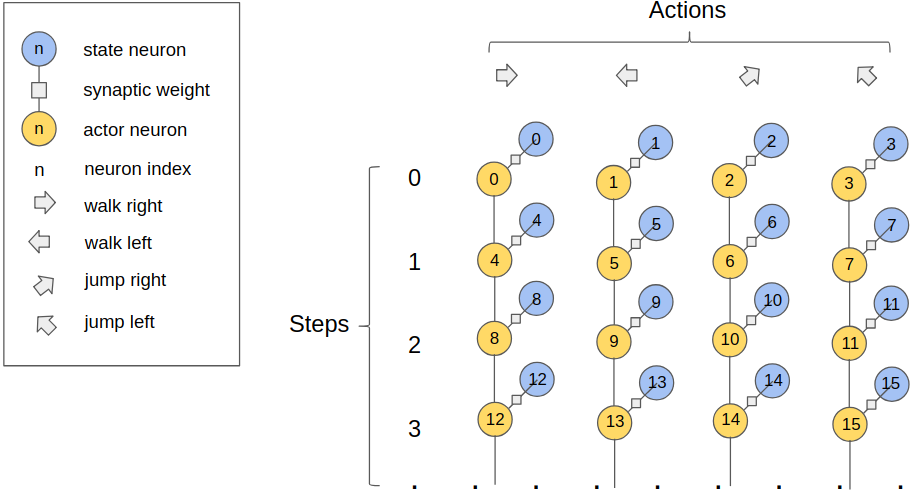
\includegraphics[width=147mm]{./neuronsWideLegend.png}
    \caption{Diagram showing how the synaptic weights between the state neurons and the actor neurons encode the policy of the agent.}
    \label{fig:stateActor}
    \end{suppfigure*}

    \subsection{The Actor-Critic learning model}

    The actor-critic model can be viewed through the framework of control theory. \textit{'The behavior of the controlled system is influenced
    by disturbances, and feedback from the controlled system to the controller provides information on which the control signals can depend'} (Barto, 1995).

    Figure \ref{fig:potjansArchitecture} shows a diagram adapted from Sutton \& Barto, 1998, of an actor-critic architecture implemented by Potjans et al., 2009. The actor supplies an action to the environment based on its policy. As a result of the action, a new state is entered and the environment transmits the new state information to the actor and critic. The critic evaluates whether the new state is better or not and emits an error signal used to update both the value function and the policy. The error signal is based on the concept of \textit{"temporal difference learning"} (TD) (Sutton et al., 1998), which aims to estimate and predict the outcome of actions without waiting for the final outcome.

    \begin{figure}[ht!]
    \centering
    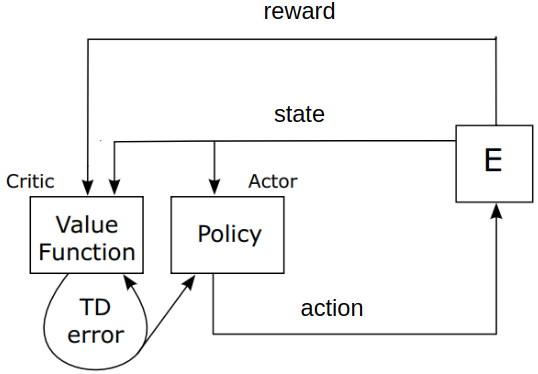
\includegraphics[width=80mm]{./actorCriticDiagram.png}
    \caption{Actor critic architecture (Potjans et al., 2009)}
    \label{fig:potjansArchitecture}
    \end{figure}

    In the case of our game, the agent executes actions and the environment sends both the agent and the critic the information regarding the resulting state. The critic then evaluates the results and modifies both the policy of the agent and its own internal information, and then the game is restarted. This counts as one learning episode, and the agent in the next episode will now use the policy learned and the signal given by the environment to execute new actions, change its behaviour if previous ones have been modified, exploit rewarded actions and explore new ones if mandated by the critic. 
    
    This cycle is repeated, the agent aquires a policy and the critic optimises it until the game is solved.

    \subsubsection{The agent}

    \textit{'A learning agent must be able to sense the state of its environment to some extent and must be able to take actions that affect the state.'} (Sutton et al., 1998). There are 4 meaningful actions that the agent could take in the case of our game: walking right, left, jumping right or jumping left. Furthermore, we need to keep track of the action that should be taken at each step in time (i.e. for each state). These actions across steps are represented by two populations of LIF neurons, a pre-synaptic state population and a post-synaptic actor population, illustrated in Figure \ref{fig:stateActor} as blue and yellow respectively.
    
    \newpage
    The neurons in each population are connected one-to-one by synapses implementing the STDP model. The populations are split so that the index of each neuron describes the action and step that they correspond to. For example, for \textit{n} possible actions, the modulo and quotinent of the division by \textit{n} of the index of the neuron that fired would give the action index and step index respectively. So, in our example, if we have 4 possible actions and the agent gives out a sequence of neurons that spiked such as [0, 6, 8, 12], this would translate into [walk right, jump right, walk right, walk right] which would be executed in that order. Furthermore, neurons representing actions at each step are connected to their analogues for future steps (the connections are seen as the vertical lines in Figure \ref{fig:stateActor}), increasing their corresponding weights and mimicking the behaviour where actions executed in the present will increase the probability that the same actions will be executed in the future.

    \textit{'The synaptic weights between the state neurons and the actor neurons encode the policy of the agent'} (Potjans et al., 2009). Each action at each step has a weight associated with it, implemented by the STDP synapses between the state and actor populations. For any particular step, the action with the greatest weight is retrieved from the network by using first-spike coding, where the neuron with the greatest synaptic weight is the most likely to fire first (VanRullen, 2005). \textit{The stronger the synaptic weights between the activated state and a given actor
    neuron, the greater the probability that it will fire first. Whichever actor
    neuron fires first in response to the activation of a state is interpreted by
    the environment as the chosen action.'} (Potjans et al., 2009). To achieve this, a population of spike injector neurons is connected to the state population, sending spikes to all neurons for each step (as seen in Figure \ref{fig:firstSpike}), while the spike receivers wait for the first spike generated by the actor neurons that will translate into an action to be executed on the environment.

    \setcounter{figure}{5}

    \begin{figure}[ht!]
    \centering
    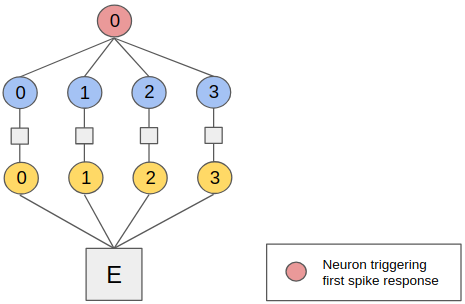
\includegraphics[width=90mm]{./firstSpike.png}
    \caption{Spike injector neuron triggering first spike response for first step (step 0) \label{overflow}}
    \label{fig:firstSpike}
    \end{figure}

    \setcounter{figure}{6}

    \newpage
    With these techniques, no other data structure is used in order to store the information about the policy of the agent, which gives a biologically accurate model for how memory might work in the brain by using synaptic plasticity.

    Figure \ref{fig:potjansImplementation} shows a diagram of the neuronal implementation of the actor-critic architecture given by Potjans et al., 2009, by which this implementation was inspired.

    \begin{figure}[ht!]
    \centering
    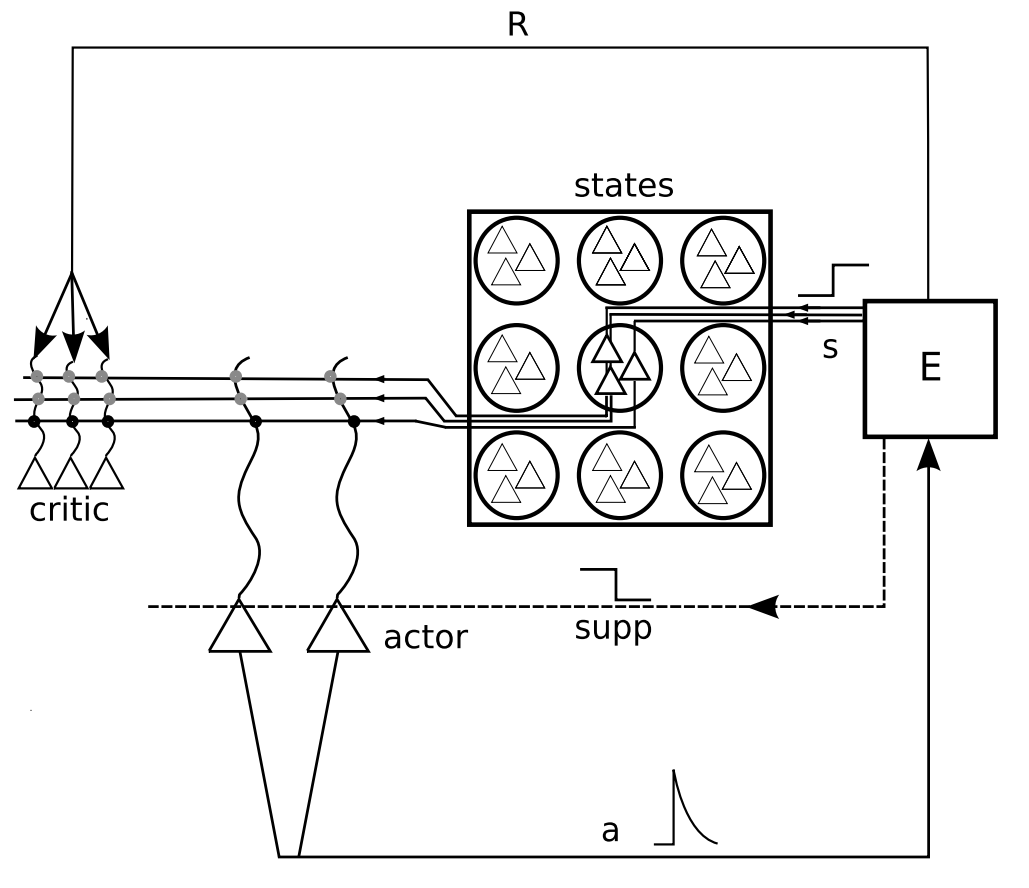
\includegraphics[width=80mm]{./implementation.png}
    \caption{Neuronal implementation of the actor critic architecture (Potjans et al., 2009)}
    \label{fig:potjansImplementation}
    \end{figure}

    \setcounter{suppfigure}{8}
    \begin{suppfigure*}[b]
    \center
    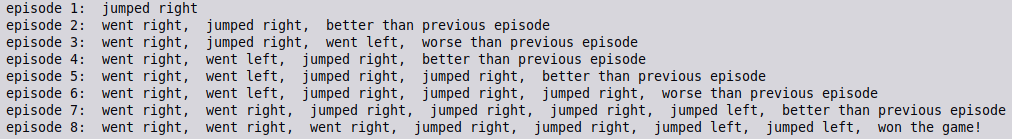
\includegraphics[width=180mm]{./history.png}
    \caption{Logs showing the activity of the agent and the evaluation of the critic over learning episodes}
    \label{fig:history}
    \end{suppfigure*}

    \subsubsection{The environment}

    To model the state, as in the \textit{'signal conveying to the agent some sense of "how the environment is" at a particular time'} (Sutton et al., 1998), a Computer Vision system is used. An external Python library which uses template matching takes a template of how the agent and goal look like and identifies their coordinates in a screenshot of the running game. Multiple screenshots are taken and cross-referenced in order to increase the reliability of the system, handling side effects such as the character unexpectedly changing its location after the learning episode has ended (for example, when it did not finish falling off a ledge) or the library failing to reliably detect the positions of the character and the goal. There is a population of spike injectors corresponding to the environment which is connected to the state neurons described in the previous section. Depending on where the agent is at the end of a particular episode the environment sends to the agent a signal corresponding to the next action that will get it directly to the goal, which will then be the action executed in the next learning episode. At the same time, the environment sends the information to the critic which compares the results of the previous learning episode to the results of the current one.

    \subsubsection{The critic}

    As the critic gets the information from the environment regarding the progress of the agent towards the goal, it compares it to the progress made in the last state of the previous learning episode and alters the weights of the corresponding actions via STDP to reward or punish those actions. This is propagated to all the actions that happened in that learning episode, with the effect decreasing linearly and the most recent action being influenced the most.

    If the agent continually does not make progress (i.e. it does not get closer to the goal), the critic enables an exploration phase in which the agent will try a random action rather than the action suggested by the environment until progress is made.

    Actions are grouped into classes depending on whether they produce a similar result (i.e. they take the character in the same direction), so that in the exploration phase the agent tries a random action from a class different from the one that was unsuccesfully executed previously.

    Figure \ref{fig:learning} shows the synaptic weights of 2 possible actions (walking right versus jumping right) that the agent could take as its second move, recorded during a simulation on the first level of the game. In this case, the agent chose to walk right at the second step in the first learning episode. At the end of it, the critic observed that the agent got closer to the goal then it previously was, so it rewarded this move and the synaptic weight increased. For the second learning episode, however, this choice turned out to eventually lead to the agent not making progress, so it has been punished, the weight becoming lower than the option of jumping right at the second step. Over time, this option stabilised as the optimal choice, and we can see that the weights of those two actions begin to diverge.

    The actual values of the weights are not as important as the relative relationship between them. For the actor-critic model, we are only interested in the action with the greatest weight, regardless of its value.

    \begin{figure}[ht!]
    \centering
    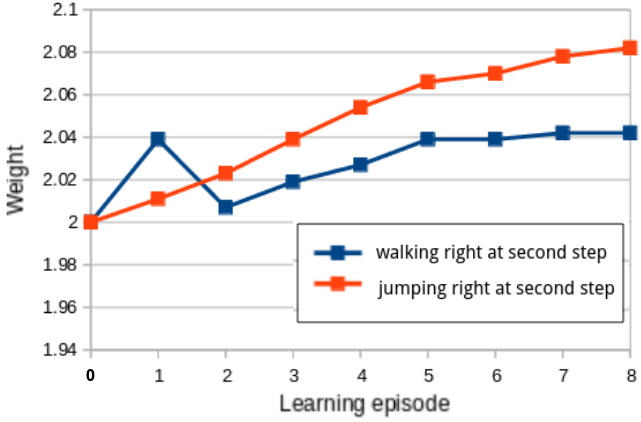
\includegraphics[width=84mm]{./learning.png}
    \caption{Weight of 2 possible actions for a given step across learning episodes}
    \label{fig:learning}
    \end{figure}
    \setcounter{figure}{9}

    Pseudocode describing a high level version of the implementation of the whole actor-critic model developed in this project is provided in Appendix A.

    Figure \ref{fig:history} shows a log taken from the running simulation of the model for the first level of the game, describing the history of the learning episodes, with the moves that the agent executed at each of them, and the analysis of the critic for each episode. We can observe that, as the critic gives feedback on the progress across episodes, the policy of the agent is altered via STDP across its whole history through the backpropagation of feedback over moves in the past.
    
    \begin{figure*}[b]
    \center
    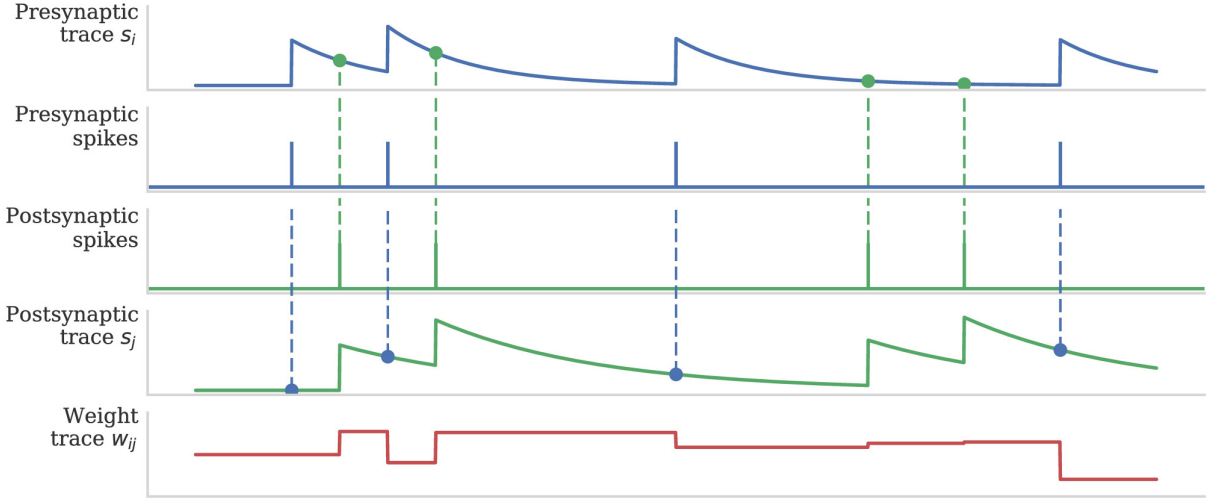
\includegraphics[width=160mm]{./spikeTraces.png}
    \caption{Calculation of weight updates using pair-based STDP traces. After Morrison et al. (2008)}
    \label{fig:spikeTraces}
    \end{figure*}

    \section{Experimentation}

    This section describes some of the behaviour and limitations of the SpiNNaker platform, and the progression of the ways in which the project was implemented, explaining their drawbacks and alternatives. The different options for customising the parameters of the network are explained and explored, presenting the results and reasoning behind them.

    \begin{figure*}[b]
    \center
    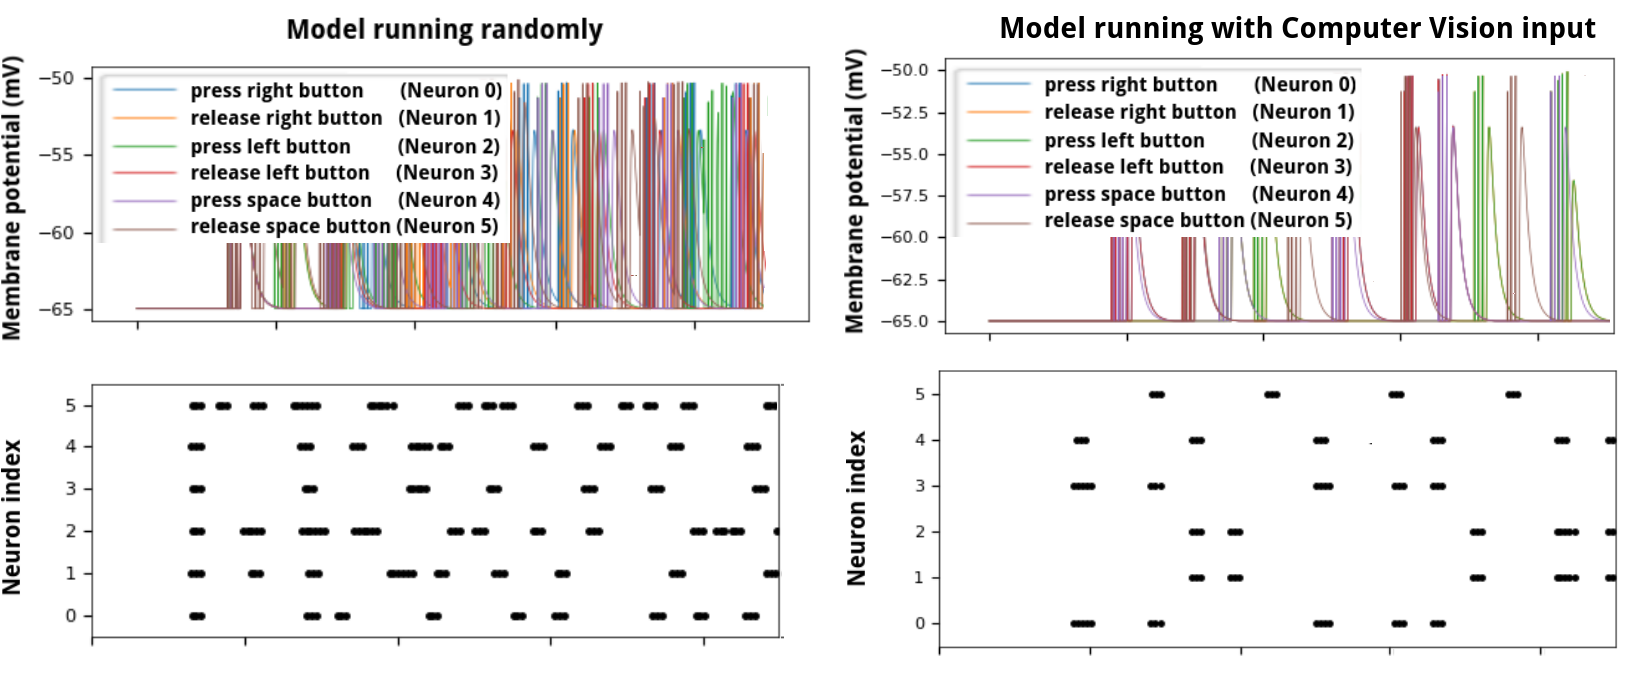
\includegraphics[width=185mm]{./diag12Long.png}
    \caption{Diagrams showing the model running randomly versus the model running with input from the environment via the Computer Vision implementation. The top diagrams are traces of the membrane voltages of neurons, while the bottom diagrams are raster plots of spiking events corresponding to actions triggered by threads running in parallel}
    \label{fig:diag}
    \end{figure*}

    \subsection{Limitations of the SpiNNaker platform}

    The \textit{run()} method of the SpiNNaker simulation is a blocking operation, and methods such as \textit{getWeights()} cannot be executed until the simulation has been completed. This is because the synaptic weights represent a large amount of data compared to the sparse spiking events, and accessing it could potentially flood the network and likely destroy the simulation (Stokes, 2016).

    It is possible however to call \textit{run()} a number of times, extracting data between each run and passing it to an external simulation (SpiNNaker Manchester, 2016). An initial version of this project would have each learning episode in a separate call of the \textit{run()} method, with simulations being started for each of them. The matrix of synaptic weights would thus be extracted between runs, and the actions with the greatest weights could be selected. The resulting spikes given by the critic and the environment would then be put on the event database as callbacks which would be executed during the run of the next learning episode.
    
    With the current implementation of sPyNNaker, if the memory requirements for a simulation cannot be met, it is split furthermore into steps where it is executed for a shorter amount of time, paused, processed and then resumed repeatedly until it completes. This method, however, repeatedly instantiates the callbacks which were intended to be only ran once during the simulation, executing them at each step, a hidden behavior that might be an error in the current implementation.
    
    Starting a simulation is a relatively lengthy process, taking around 10 seconds. A later version of the project would run the model in a separate execution thread to the thread running the simulation. The critic and environment would now inject spikes into the network during the simulation with the use of spike transmitters instead of callbacks. For the weights, we are not interested in the actual values as much as we are interested in which synapse has the greatest value relative to the others. First spike coding (VanRullen, 2005), suggests that the stronger the synaptic weight for a given post-synaptic neuron, the greater the probability that it will fire first. By injecting spikes to groups of neurons corresponding to actions over steps and recording the indices of the first neurons that spike, we can determine the synapses with the greatest weights without interrupting the run, removing the great overhead of repeatedly initialising simulations.

    \subsection{Exploring different neuron properties}

    Figure \ref{fig:spikeTraces} shows how voltage traces are sampled to compute STDP weight updates depending on the order of spiking events. Potentiation is calculated at each post-synaptic spike by sampling the pre-synaptic trace (green circles) to obtain a measure of recent pre-synaptic activity, while depression is done by sampling the post-synaptic trace (blue circles) (Mikaitis et al., 2018).

    PyNN provides a number of parameters that can be customised to modify the properties of neurons and their connections in order to have control over the behaviour and timings of the processes shown in Figure \ref{fig:spikeTraces}. In the case of the LIF model, among other properties are the capacitance of the neuron, the refractory period and the excitatory input current decay time-constant. In the case of the projections describing the STDP synapses between neurons, we can modify elements such as the exponential decay of the size of the weight update for both the potentiation and the depression of neurons.

    For our model, because there is some latency between the spikes sent by the critic in a specific order to either depress or potentiate a synapse, the current decay of the neurons has been decreased to accomodate this and give time for the spikes to arrive and modify the weights. In the case of Figure \ref{fig:spikeTraces}, this would show as a slower slope for the decay of the synaptic traces.
    
    Furthermore, to stop pre-synaptic state neurons from generating multiple successive post-synaptic actor spikes, the refractory period of the actor population has been increased in the final implementation of the project. This gives more consistent results in the case of generating first-spike events which are needed to decode the policy of the agent.

    \subsection{Exploring multithreading for actions}

    One early version of the implementation had separate threads for each of the possible actions, which would operate independently and concurrently. This method would prove to not be viable as the effects of the separate actions being executed concurrently would not be consistent over learning episodes due to variations in the latencies of these threads. This would hinder the ability of the model to reliably exploit rewarded policies learned in previous episodes. Furthermore, this method would not scale for a greater number of actions. The final implementation abandons this version in favour of executing actions sequentially in one thread, which improved the results and the consistency of the model's behaviour across learning episodes.
    
    For the multithreaded version initially however, more actions were implemented, corresponding to individual button presses and releases. These were later merged and modified to result in the final, more effective actions presented earlier (walk right, left, jump right and jump left). Figure \ref{fig:diag}, recorded from an early version of the multithreaded implementation, shows the differences between the model running randomly and the model running with the input from the environment via the Computer Vision implementation for the first level of the game. On the raster plots of spiking events we can see that for the model running randomly, the actions are arbitrary, and in the game they do not produce any meaningful results. For the model running with the input of the environment through the Computer Vision implementation, however, we can see that the actions are much more structured and consistent, which translates into genuinely effective moves in the game. The model, however, gets stuck in a loop corresponding to a local optimum of the specific level, the path of which is blocked by an obstacle. We can see this in the repetition of the pattern in the raster plot. To combat this, the concept of a critic has to be introduced in order to detect the lack of progress over the iterations of the agent and adjust its policy accordingly.

    \section{Future development}

    This chapter presents various ideas and opportunities for further improving the model. These methods have been explored but not implemented in the final version of the project, either due to their complexity or due to the relatively small effect that they would have on the overall effectiveness of the model.

    \subsection{Improving the critic}

    \subsubsection{Detecting unproductive moves}

    It is possible that the agent solves the level in a sub-optimal way, for example by executing moves at one point that do not contribute to the solution (such as going left and right repeatedly thus cancelling those actions out). An \textit{'adaptive critic'} (Barto, 1995) would improve its evaluative feedback by maximising a \textit{'weighted sum of all future primary reinforcement values'} (Barto, 1995). The sensory input of the critic, however, would need to be rich enought so that it can extract from its history predictions for situations that have similar \textit{"futures"}.

    \subsubsection{Preserving the optimal sections of the policy}

    Currently, the backpropagation of the critic's feedback could alter moves in the past that were otherwise optimal. To combat this, the critic could identify synapses corresponding to sections of the agent's policy that are optimal and \textit{"freeze"} them so that they are not altered and will always be exploited by the agent.

    \subsubsection{Varying the critic feedback frequency}

    Currently, the critic interrupts the activity of the agent uniformly across the level in order to evaluate its policy and modify it. The critic's feedback, however, might not be always needed during the agent's activity on easier sections of the level (for example on long platforms where the only suitable action is going in one direction, which the behaviour of the agent will execute optimally without the need of the critic's feedback). To make the model more efficient and have the agent converge to a solution faster, the critic could identify the parts of the level where it thinks the agent would require more frequent evaluation, increase the rate at which it will give feedback for that portion and decrease it for sections that seem straightforward for the agent. To achieve this, the critic could look at the history of how easy the agent made progress over previous sections of the level, and identify sections with similar properties that it will adapt its feedback frequency for in the future.

    \subsubsection{Mapping reoccurring actions to a single neuron}

    Some sequences of actions reoccur over the course of the agent's activity, but they require a neuron each. To optimise memory, the critic could identify those reoccurring actions and map the whole sequence to a single neuron, so that the whole routine would be triggered by that neuron.

    \subsection{Connecting hardware}

    All the spiking events that are produced by the system or injected into it are transmitted and received at UDP ports. In the case of this project, the Computer Vision implementation senses the environment and injects corresponding spikes into the network, while the system produces spikes that are recorded and translated into button presses. Rather than having a Computer Vision system recording the game, we could attach actual environmental sensors (such as proximity detectors, cameras etc.) that communicate to the network, placed on a robot trying to solve a real world puzzle. Instead of spikes producing virtual button presses, the spike receivers could be connected to actuators that execute actions in the environment (for example through servomotors).

    \section{Evaluation}

    This section presents the results of the model when applied to solve levels of the game. It describes the speed with which actions are decoded, the scalability of the implementation regarding both the low number of neurons and learning episodes required to reach solutions, the consistent performance when faced with more challenging levels and the resilience to imprecisions in the configuration of the actions.

    \subsection{Performance}
    
    The goal of the project is to produce a model that would solve the levels in a small number of learning iterations, for a total amount of time that would be short enough that this method could be applied to real world applications where either time resources for training are limited, or where software cannot accurately simulate the real world behaviour of the system for training.

    For the task of the first level illustrated in Figure \ref{fig:firstLevel}, across a couple of hundreds of tests, the model converges to a solution in an average of 11 learning episodes ($\sigma$ = 1.5), taking around 2 minutes and 6 seconds ($\sigma$ = 24s) to successfully pass each test. The game was not simulated or sped up, so these are benchmarks of the behaviour of the model in real time. For this level, the model has been configured to have enough neurons to execute a maximum of 12 steps, and it successfully finds the solution to the level before it runs out of neurons around 80\% of the time when executing the tests.

    \subsection{Latency}

    To decode an action, the speed at which the first spike event propagates across the network from the moment it is emitted by the spike transmitter to the moment it is recorded by the spike receiver is around 5 to 7 milliseconds. This would be a promising latency between a sensor generating a spike and an actuator executing a move for a real world application.  With one population per step (i.e. per row of state neurons in Figure \ref{fig:stateActor}), all first spike triggers needed to decode the actions could be sent at the same time in parallel, decoding all the actions for all the steps in 5 to 7 milliseconds. Each SpiNNaker core can only model 1 population however, so scalability for the number of steps needed to solve a level (i.e. the number of moves required) is limited by the number of cores that the platform running the simulation has. The high speed of decoding a large number of possible actions over a large number of steps with limited energy consumption could give the opportunity of developing robotic prostethics able to execute complex actions requiring fine movements. The biological accuracy of the implementation could also be the basis for interfacing with the nervous system, possibly training the model through a combination of neural inputs from the user and inputs from sensors monitoring the environment.

    \subsection{Scalability}

    The number of neurons required to solve a level is a function of the number of steps that the agent needs to take in order to solve it, times the number of possible actions (i.e. the number of rows times the number of columns in Figure \ref{fig:stateActor}), resulting in the following formula:

    \begin{center}
        \textit{N = S $\times$ A $\times$ 4 + S}
    \end{center}

    Where \textit{N} is the number of neurons required to solve a level, \textit{S} is the number of steps required to solve that level and \textit{A} is the number of possible actions the agent could choose from at each step. We need \textit{S $\times$ A} neurons for the state and actor populations and the populations corresponding to spike injector neurons for the critic and evironment (resulting in 4 populations). To decode the actions, a spike injector neuron is connected to the state neurons at each step, this population resulting in an additional \textit{S} number of neurons.

    Furthermore, the agent only executes a move for 1 additional step per learning episode (i.e. it executes 1 move in the first learning episode, 2 moves in the second one and so on) meaning that the number of learning episodes required to solve a level will always be equal to the number of required steps. In the case of the first level, the model was able to solve it in 12 steps by using its 4 available actions, resulting in \textit{12 $\times$ 4 $\times$ 4 + 12 = 204} neurons used.

    The model, however, can solve increasingly more difficult levels such as the one illustrated in Figure \ref{fig:complexLevel}, where only 25 learning episodes over the course of around 7 minutes were needed. This results in \textit{25 $\times$ 4 $\times$ 4 + 25 = 425} neurons required for this level. In addition to the platforms that the character needs to navigate (and \textit{"wall jump"}) around, this level also introduces sawblades, where by touching them the character is \textit{"killed"} and sent back to the starting point at the bottom of the level. Despite of this, the model handles this level quite well.

    \begin{figure}[ht!]
    \centering
    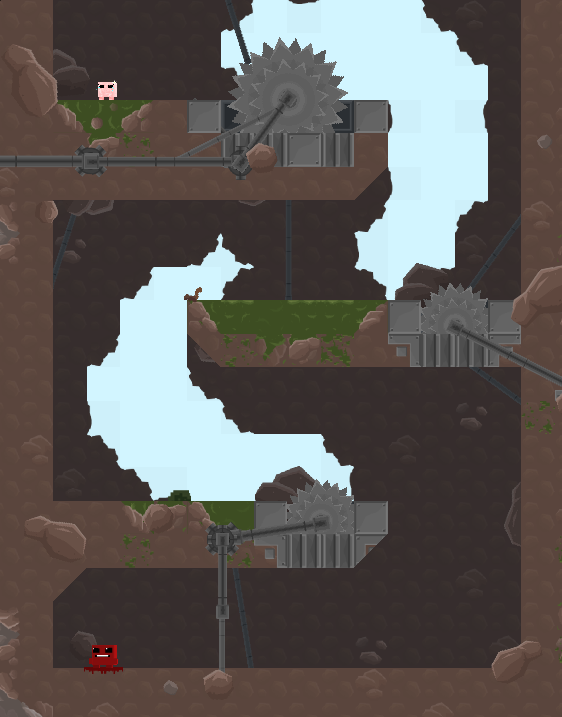
\includegraphics[width=81mm]{./bladeLevelLong.png}
    \caption{More complex level, with an increased number of platfroms and where sawblades placed on each platform \textit{"kill"} the player and bring him back to the starting point}
    \label{fig:complexLevel}
    \end{figure}

    Because the model can solve these levels in such a low number of learning episodes compared to tabular methods such as Q-Learning or SARSA, it makes it suitable for real world applications where the behaviour cannot be simulated to speed up learning and generate the thousands of episodes that these methods usually require.

    \subsection{Sensitivity}

    The most important variable that the model could be sensitive to is the configuration of the actions. Each action corresponds to a button press, however holding the button for a different amount of time would result in a widely different action. Some sort of heuristic needs to be taken into consideration when configuring the actions, for example the type of actions that humans take while playing the game and for how long these actions are held. Currently, each action (i.e. button press) is held for 0.5 seconds. Increasing the duration that the moves are held for by up to 30\%, however, does not affect the performance of the model, demonstrating that it is resilient to imprecisions or arbitrary configurations in the actions.

    \section{Project management and planning}

    \textit{'Working software is the primary measure of progress'} (Beck et al., 2001). Following the principles of Agile software development, even from the earliest stages of the project the aim has always been to produce fast prototypes of working elements of the implementation.

    The SpiNNaker group provides a laboratory manual describing the configuration of the system and the supporting Python libraries (SpiNNaker Manchester, 2016) and various implementation examples on the GitHub repository of the group (Spinnaker Manchester, 2019). These resources would provide instructions and inspiration for achieving basic pieces of functionality, such as setting spiking callbacks before a simulation, using the spike transmitters and receivers to inject and record spikes, producing plots of the activity of the system and so on.

    These resources were used and explored to produce pieces of the functionality that lead to the ideas and implementations used in the project. The proccess followed the model of iterative and incremental development, where functionality was gradually added and improved, slowly discovering the direction of the project over the course of implementation.

    Throughout the entire development, the model has been run on the game and evaluated, and functionality has been gradually added to reach the goal of reliably and efficiently solving the tasks. Initially, the model was ran with random inputs, with unsuccesful results towards solving the game. A basic implementation of an enviromental input via a Computer Vision system was added, producing more consistent behaviour that however still did not solve the game. Extensive research into learning methods has been made, finding the Actor-Critic learning model which could be suitable for a biologically accurate implementation of the project. The critic has been added to the network, altering the behaviour of the previously implemented agent, with promising results that managed to solve the game. The rest of development time was then spent on exploring ways to improve this model to solve the game more reliably, and to enable it to solve increasingly harder levels.

    The aim was to produce a working, demoable version of the project by the end of the first 3 months of development, which was achieved in the form of the model trying to solve the game with the use of the environmental input. The following month was used to introduce and implement the critic, and the rest of development time (around 2 months) was used to improve the model, experiment with different architectures and evaluate it.

    \subsection{Personal development}

    This project provided the opportunity of getting a practical experience with state-of-the-art neuromorphic computing technologies, involving both elements of extensive research, implementation and evaluation. Aspects of Agile software development were practiced with succesful results, and skills regarding project management and planning were improved.
    
    \section{Conclusion}

    An Actor-Critic learning agent on the SpiNNaker neuromorphic computing plaform was explored, implemented and evaluated, building upon concepts and architectures described in a number of research papers. Novel techniques specific to the SpiNNaker architecture are introduced to achieve this model, while also describing ideas for new, biologically accurate information storing methods and future develoment.

    The project provides a scalable and reliable model for reinforcement learning, its concepts and implementation possibly being able to be used to improve the development and biological accuracy of energy efficient technologies such as robotic prostethics or mobile robotics able to solve complex, faster than real time tasks.

    In conclusion, the project has been a success, both regarding the results generated and the breadth of new concepts, techniques and tools learned.

    \section*{Acknowledgements}
    \addcontentsline{toc}{section}{\protect\numberline{}Acknowledgements}

    I would like to thank my supervisor Steve Furber for the continuous support over the course of the year and for the guidance that helped me to organise, implement and present my project. I would also like to thank Peter Bogdan for helping me aquire and set up the tools necessary to start development, and for pointing me to the most important papers and books that this project is primarily based on.
    
    \onecolumn

    \newpage
    \addcontentsline{toc}{section}{\protect\numberline{}Appendices}
    \section*{Appendix A}
    \addcontentsline{toc}{subsection}{\protect\numberline{}Appendix A}

    \begin{lstlisting}[]

        Restart the game
        Get first action via input from environment
        Repeat (for each episode):
            Repeat (for each step of episode + 1):
                If this is the last step:
                    Get next best action from environment
                    Send spikes to agent to encode it
                Else:
                    Decode actions from agent via first spike
            Execute decoded actions
            If exploring:
                Don't execute action given by environment for last step
                Execute another random action
            Else:
                Execute action given by environment for last step
            Have critic get input from environment
            If better than previous episode:
                Repeat (for each command in policy, descending):
                    Potentiate the synapse corresponding to command
                    Decrease potentiation rate
            Else:
                Repeat (for each command in policy, descending):
                    Depress the synapse corresponding to command
                    Decrease depression rate
            If continually not making progress:
                Enable exploration
            Else:
                Disable exploration
            Restart the game
    
    
    \end{lstlisting}    
        
    \newpage
    
    \section*{References}
    \addcontentsline{toc}{section}{\protect\numberline{}References}

    Barto, A. G. (1995) \textit{Adaptive Critics and the Basal Ganglia} \\[-3pt]

    \noindent
    Beck, K., Beedle, M., van Bennekum, A., Cockburn, A., Cunningham, W., Fowler, M., Grenning, J., Highsmith, J., Hunt, A., Jeffries, R., Kern, J., Marick, B., Martin, R., C., Mellor, S., Schwaber, K., Sutherland, J., Thomas, D. (2001) \textit{Manifesto for agile software development} \\[-3pt]

    \noindent
    Benjamin, B. V., Gao, P., McQuinn, E., Choudhary, S., Chandrasekaran, A. R., Bussat, J.-M. K., et al. (2014) \textit{ Neurogrid: a mixed-analog-digital multichip system for large-scale neural simulations} \\[-3pt]

    \noindent 
    Brette, R., Rudolph, M., Carnevale, T., Hines, M., Beeman, D., Bower, J. M., et al. (2007) \textit{ Simulation of networks of spiking neurons: a review of tools and strategies} \\[-3pt]

    \noindent    
    Furber, S. B., Galluppi, F., Temple, S., and Plana, L. A. (2014) \textit{The SpiNNaker project} \\[-3pt]
    
    \noindent    
    Furber, S. B., Lester, D. R., Plana, L. A., Garside, J. D., Painkras, E., Temple, S., Brown, A. D. (2013) \textit{Overview of the SpiNNaker system architecture} \\[-3pt]

    \noindent
    Hebb, D. O. (1949) \textit{The Organization of Behavior} \\[-3pt]

    \noindent    
    Klopf, A. H. (1982) \textit{The Hedonistic Neuron: A Theory of Memory, Learning, and Intelligence} \\[-3pt]

    \noindent
    Maass, W. (1996) \textit{Networks of Spiking Neurons: The Third Generation of Neural Network Models} \\[-3pt]

    \noindent
    Markram, H., Lubke, J., Frotscher, M., Sakmann, B. (1997) \textit{Regulation of synaptic efficacy by coincidence of postsynaptic APs and EPSP } \\[-3pt]

    \noindent
    Mead, C. A. (1990) \textit{Neuromorphic electronic systems} \\[-3pt]

    \noindent
    Mikaitis, M., Pineda García, G., Knight, J. C., Furber, S. B. (2018).  \textit{Neuromodulated Synaptic Plasticity on the SpiNNaker Neuromorphic System} \\[-3pt]

    \noindent
    Morrison, A., Diesmann, M., Gerstner, W. (2008) \textit{Phenomenological models of synaptic plasticity based on spike timing} \\[-3pt]

    \noindent
    Potjans, W., Morrison, A., Diesmann, M. (2009) \textit{A spiking neural network model of an actor-critic learning agent} \\[-3pt]

    \noindent
    Rhodes, O., Bogdan, P. A., Brenninkmeijer, C., Davidson, S., Fellows, D., Gait, A., Lester, D. R., Mikaitis, M., Plana, L. A., Rowley, A. G., Stokes, A. B., Furber, S. B. (2018) \textit{sPyNNaker: a Software Package for Running PyNN
    Simulations on SpiNNaker} \\[-3pt]

    \noindent
    Sarpeshkar, R. (1998) \textit{Analog Versus Digital: Extrapolating from Electronics to Neurobiology} \\[-3pt]

    \noindent
    SpiNNaker Manchester (2016) \textit{Sixth SpiNNaker workshop lab manuals} \\[-3pt]
    
    \noindent
    SpiNNaker Manchester (2019) \textit{https://github.com/SpiNNakerManchester/PyNN8Examples [accessed April 2019]} \\[-3pt]

    \noindent
    Stokes, A. B. (2016) \textit{Weight updates during simulation - SpiNNaker Users Group} \\[-3pt]

    \noindent
    Sutton, R. S., Barto, A. G. (1998) \textit{Reinforcement learning: An Introduction} \\[-3pt]

    \noindent
    Thorndike, E. L. (1898) \textit{Animal intelligence: An experimental study of the associative processes in animals} \\[-3pt]

    \noindent
    VanRullen, R., Guyonneau, R, Thorpe, S. J. (2005) \textit{Spike times make sense} \\[-3pt]
    
    \end{document}
    